%% Version 6.1, 1 September 2021
%
%%%%%%%%%%%%%%%%%%%%%%%%%%%%%%%%%%%%%%%%%%%%%%%%%%%%%%%%%%%%%%%%%%%%%%
% TemplateV6.1.tex --  LaTeX-based blank template for submissions to the 
% American Meteorological Society
%
%%%%%%%%%%%%%%%%%%%%%%%%%%%%%%%%%%%%%%%%%%%%%%%%%%%%%%%%%%%%%%%%%%%%%
% PREAMBLE
%%%%%%%%%%%%%%%%%%%%%%%%%%%%%%%%%%%%%%%%%%%%%%%%%%%%%%%%%%%%%%%%%%%%%

%% Start with one of the following:
% 1.5-SPACED VERSION FOR SUBMISSION TO THE AMS
\documentclass{ametsocV6.1}

%% load additional packages
\usepackage{tabularx}
\usepackage[en-GB]{datetime2} % \usepackage[en-GB,en-US]{datetime2}
\DTMlangsetup[en-GB]{ord=raise,monthyearsep={,\space}}

% Define colours to capture author contributions
\def\cred#1{{\color{red}#1}}

% TWO-COLUMN JOURNAL PAGE LAYOUT---FOR AUTHOR USE ONLY
% \documentclass[twocol]{ametsocV6.1}
%%%%%%%%%%%%%%%%%%%%%%%%%%%%%%%%
%%% To be entered by author:
%% May use \\ to break lines in title:

\title{Earth system forcing for CMIP7 and beyond}

%% Enter authors' names and affiliations as seen in the examples below.
%
%% Use \correspondingauthor{} and \thanks{} (\thanks command to be used for affiliations footnotes, 
%% such as current affiliation, additional affiliation, deceased, co-first authors, etc.)
%% immediately following the appropriate author.
%
%% Note that the \correspondingauthor{} command is NECESSARY.
%% The \thanks{} commands are OPTIONAL.
%
%% Enter affiliations within the \affiliation{} field. Use \aff{#} to indicate the affiliation letter at both the
%% affiliation and at each author's name. Use \\ to insert line breaks to place each affiliation on its own line.

%\authors{Author One,\aff{a}\correspondingauthor{Author One, email@email.com} 
%Author Two,\aff{a} 
%Author Three,\aff{b,d} 
%Author Five\thanks{Author Five's current affiliation: NCAR, Boulder, Colorado},\aff{c} 
%}
%\affiliation{\aff{a}{First Affiliation}\\
%\aff{b}{Second Affiliation}\\
%}

\authors{
	Paul J. Durack\aff{a}\correspondingauthor{Paul J. Durack, pauldurack@llnl.gov},
	Vaishali Naik\aff{b},
	Zebedee Nicholls\aff{c},
	Eleanor O’Rourke\aff{d},
	Briony Turner\aff{d},
	Carlo Buontempo\aff{e},
	Anca Brookshaw\aff{e},
	Christopher Goddard\aff{e},
	Claire MacIntosh\aff{f},
	Helene Hewitt\aff{g},
	John Dunne\aff{b}
	}

\affiliation{
	\aff{a}{PCMDI, Lawrence Livermore National Laboratory (LLNL), Livermore, California 94550, USA},
	\aff{b}{NOAA Geophysical Fluid Dynamics Laboratory (NOAA-GFDL), Princeton, New Jersey 08540, USA},
	\aff{c}{Climate Resource S GmbH, Berlin, Germany; Energy, Climate and Environment Programme, International Institute for Applied Systems Analysis (IIASA), Laxenburg, Austria; School of Geography, Earth and Atmospheric Sciences, University of Melbourne (UoM), Parkville, Victoria, Australia},
	\aff{d}{CMIP International Project Office (CMIP-IPO), ECSAT, Harwell Science and Innovation Campus, UK},
	\aff{e}{European Centre for Medium-Range Weather Forecasts (ECMWF), Bonn, Germany and Reading, UK},
	\aff{f}{European Space Agency (ESA) ECSAT, Harwell, UK},
	\aff{g}{Met Office Hadley Centre (MOHC), Exeter, UK},
	}

%%%%%%%%%%%%%%%%%%%%%%%%%%%%%%%%%%%%%%%%%%%%%%%%%%%%%%%%%%%%%%%%%%%%%
% Notes for authors - Below are a couple of relevant URLs
%
% CMIP-IPO onlyoffice file - pre-tex version
% https://office.wcrp-cmip.org/Products/Files/DocEditor.aspx?fileid=10939
%
% CMIP-IPO working folder
% https://office.wcrp-cmip.org/Products/Files/#3848
%
% AMS resources
% https://www.ametsoc.org/ams/publications/author-information/author-responsibilities-during-production/copyright-information/standard-copyright-forms/
%%%%%%%%%%%%%%%%%%%%%%%%%%%%%%%%%%%%%%%%%%%%%%%%%%%%%%%%%%%%%%%%%%%%%

\begin{document}

%% Necessary to enable compilation
\abstract{}
\centerline{{\cred{\textbf{A working draft document, dated \DTMnow}}}}
\maketitle

%%%%%%%%%%%%%%%%%%%%%%%%%%%%%%%%%%%%%%%%%%%%%%%%%%%%%%%%%%%%%%%%%%%%%
% BAMS Meeting Summary: What, When, Where box
%%%%%%%%%%%%%%%%%%%%%%%%%%%%%%%%%%%%%%%%%%%%%%%%%%%%%%%%%%%%%%%%%%%%%
\section*{Pathway to regular and sustained delivery of climate forcing datasets}
\subsection*{\textbf{What:}}
The World Climate Research Programme (WCRP) Coupled Model Intercomparison Project (CMIP) community convened to discuss progress and planning for generating climate ``forcing'' datasets for the upcoming CMIP7 project. Discussions also focused on evolving existing efforts to deliver a sustained or ``operational'' forcing data generation activity over the longer term. This aims to provide high-priority forcing datasets in a regular delivery mode to meet user needs, sustained by appropriate funding, resources, and infrastructure. 
\subsection*{\textbf{When:}}
28 October 2024 to 31 October 2024
\subsection*{\textbf{Where:}}
ECMWF, Shinfield Park, Reading, RG2 9AX United Kingdom 
\newpage

%%%%%%%%%%%%%%%%%%%%%%%%%%%%%%%%%%%%%%%%%%%%%%%%%%%%%%%%%%%%%%%%%%%%%
% SIGNIFICANCE STATEMENT/CAPSULE SUMMARY
%%%%%%%%%%%%%%%%%%%%%%%%%%%%%%%%%%%%%%%%%%%%%%%%%%%%%%%%%%%%%%%%%%%%%
% If you are including an optional significance statement for a journal article or a required capsule summary for BAMS 
% (see www.ametsoc.org/ams/index.cfm/publications/authors/journal-and-bams-authors/formatting-and-manuscript-components for details), please apply the necessary command as shown below:
%% Significance Statement (all journals except BAMS)
%\statement
%	 Enter significance statement here, no more than 120 words. See \url{www.ametsoc.org/index.cfm/ams/publications/author-information/significance-statements/} for details.
%% Capsule (BAMS only)
%\capsule
% Enter BAMS capsule here, no more than 30 words. See \url{www.ametsoc.org/index.cfm/ams/publications/author-information/formatting-and-manuscript-components/#capsule} for details.
%% * * If using twocol mode, you will need to use the commands "twocolsig" and "twocolcapsule" in place of "sig" and "capsule" to ensure that the text box correctly spans across both columns.

%%%%%%%%%%%%%%%%%%%%%%%%%%%%%%%%%%%%%%%%%%%%%%%%%%%%%%%%%%%%%%%%%%%%%
% MAIN BODY OF PAPER
%%%%%%%%%%%%%%%%%%%%%%%%%%%%%%%%%%%%%%%%%%%%%%%%%%%%%%%%%%%%%%%%%%%%%
%% In all cases, if there is only one entry of this type within the higher-level heading, use the star form: 

Preparation for the next phase of coordinated Earth system model experimentation, the Coupled Model Intercomparison Project phase 7 (CMIP7), is well underway. To finalize experiment protocols and begin simulations, ``forcing'' datasets must be generated and provided to modeling groups. These forcing datasets have wider utility across numerical weather prediction (NWP), reanalysis, initialized predictions, and downscaling using regional models. \\ 
\\
A broad international group addressing this need met in Reading (UK) on 28-31 October 2024 for the workshop ``Pathway to regular and sustained delivery of climate forcing datasets''. The meeting had two goals: 1) to evaluate/discuss the latest climate-forcing dataset status in preparation for CMIP7 (see Figure 1), and 2) to plan for the future, recognizing currently limited support for forcing dataset production. These goals were outlined to ensure consistent dataset delivery, enable sustained research, and facilitate the science needs of society, serving CMIP7 and beyond.

\section*{What are ``Earth system forcings''}
% \subsection*{First secondary heading}
% \subsubsection{First tertiary heading}
Earth system changes result from natural and human modulation of atmospheric constituents (solar irradiance changes, emissions of reactive gases and aerosols, volcanic eruptions, greenhouse gases, etc), land use, and other Earth system component changes. These natural or anthropogenic drivers are termed ``forcing'' agents because they drive (i.e., force) changes in the Earth system. Their sources and roles in the Earth system can vary greatly, from so called ``short-lived'' climate forcers (SLCFs), to changes in the more persistent greenhouse gas concentrations or variations in solar activity. As Earth System Models (ESMs) have become more complex and complete, the requirements and descriptive criteria for observed ``forcing'' have increased.

\section*{Who we are}
The workshop attracted a broad audience, with more than 150 registered participants from 71 institutions and 23 countries. Held in-person and virtually, the workshop allowed attendees across multiple time zones to participate remotely, ensuring early starts for some and broad engagement. The community represented a wide swath of climate-interested folks, growing markedly in recent years. Attendees included the dataset providers, modeling group representatives, a growing list of downstream forcing- and model-data users, representatives from interested funding agencies, policymakers, and private sector participants.

\section*{Earth system forcings, the next generation}
For CMIP7, we built on CMIP6 momentum \citep{durack_toward_2018}. The CMIP Forcings Task Team (the ``team'') was established in October 2022 to assess the state of climate forcings for meeting the needs of the upcoming CMIP7, comprising researchers generating forcing data, modeling group representatives, and broader community stakeholders.

The team set out to develop next-generation datasets on a tight timeline (see Figure 1), meeting the goal of having prototype data available for review by late 2024. Table 1 briefly describes next-generation datasets.


\begin{table*}[ht]
	\renewcommand{\arraystretch}{1.5}
	\renewcommand\tabularxcolumn[1]{m{#1}}% for vertical centering text in X column
	\scriptsize
	\centering
	\caption{Overview of next-generation historical forcing datasets now available for CMIP7.}
	\begin{tabularx}{1\textwidth} {
		| >{\centering\arraybackslash\hsize=.22\hsize}X
		| >{\centering\arraybackslash\hsize=.37\hsize}X
		| >{\centering\arraybackslash\hsize=.16\hsize}X
		| >{\centering\arraybackslash\hsize=.25\hsize}X | }
	\hline
	\textbf{Dataset} & \textbf{Description} & \textbf{Temporal range} & \textbf{Dataset identifier; Versions - initial release; latest (if revised)} \\
	\hline
	\multicolumn{4}{l}{\textbf{Forcing data prepared for use in the CMIP7 DECK experiments}} \\ \hline
	Anthropogenic emissions & Emissions of short-lived climate forcers (SLCFs; methane, aerosols and their precursors, ozone precursors), CO$_{2}$ and N$_{2}$O & 1750-01 to 2023-12 (monthly) & CEDS-CMIP-2025-03-18; Nov 2024/2024-10-21; 2025-04-18 \\ \hline
	Biomass burning emissions & Emissions from biomass burning, particularly fire. A portion of the emissions can be identified as a feedback, driven by observed warming & 1750-01 to 2023-12 (monthly) & DRES-CMIP-BB4CMIP7-2-0; Oct 2024/1.0; 2.1 \\ \hline
	Land use change & Land use changes between natural and anthropogenic use states, including multiple forest, grazing and functional types, along with urban use & 850 to 2024 (annual) & UofMD-landState-3-1-1; Oct 2024/3.0; 3.1.1 \\ \hline
	Greenhouse gas concentrations & Major atmospheric well-mixed greenhouse gas concentrations (WMGHGs), CO$_{2}$, CH$_{4}$, N$_{2}$O, along with Ozone Depleting Substances (ODSes), hydrofluorocarbons (HFCs) and other Montreal Protocol monitored species & 0001-01 to 2022-12 (monthly) & CR-CMIP-1-0-0; Aug 2024/0.2; 1.0.0 \\ \hline
	Stratospheric volcanic SO$_{2}$ emissions and aerosol optical properties & Stratospheric SO$_{2}$ aerosol emissions from volcanic events, providing location and injection height; and derived volcanic aerosol optical properties for models without interactive volcanic emission injections & 1750-01 to 2023-12 (monthly) & UOEXETER-CMIP-2-0-0; Sep 2024/1.1.3; 2.2.1 \\ \hline
	Ozone concentrations & Ozone concentrations simulated as consistent with other historical forcings & 1850-01 to 2023-12 (monthly) & FZJ-CMIP-1-0; Expected Aug 2025 \\ \hline
	Nitrogen deposition & Nitrogen deposition estimates due to atmospheric chemical processing of NO$_{x}$ and NH$_{3}$ & 1850-01 to 2023-12 (monthly) & FZJ-CMIP-1-0; Expected Aug 2025 \\ \hline
	Solar irradiance & Incoming short-wave solar radiation, representing solar cycle variability & 1850-01 to 2023-12 (monthly) & SOLARIS-HEPPA-CMIP-4-6; Jul 2024/4.2; 4.6 \\ \hline
	SSTs and sea-ice & Sea surface temperatures (SSTs) and polar sea ice concentrations. Used in the atmosphere-only experiment (amip) & 1870-01 to 2022-12 (monthly) & PCMDI-AMIP-1-1-9; May 2023/1.1.9 \\ \hline
	Aerosol optical properties & Aerosol optical properties based on the simple plume parameterization. These properties infer the radiative impact of aerosols in models that do not simulate them from emissions & 1850-01 to 2020-12 (monthly) & SPv2.1; Dec 2024/SPv2\_20241218; SPv2.1 \\ \hline
	\multicolumn{4}{l}{\textbf{Forcing data prepared for use in the CMIP7 Community MIP experiments (Target activity included in parentheses)}} \\ \hline
	Mineral dust aerosols (AerChemMIP2) & Reconstruction-based observed estimates of increased aeolian dust, largely from Asia and North Africa  & 1850 to 2000 (annual) & UCLA-1-0-2; Feb 2025/2025-02-12; 1.0.2 \\ \hline
	Atmospheric CO$_{2}$ carbon isotopic history (C4MIP) & Reconstruction-based observed estimates of well-mixed CO$_{2}$ isotopic composition for delta13 and delta14 & 1700 to 2023 (annual) & ImperialCollege-3-0; May 2025/3.0 \\ \hline
	\end{tabularx}
\label{tab:t1}
\footnotesize{For the latest information and available data, see \url{https://input4mips-cvs.readthedocs.io/en/latest/dataset-overviews}.}
\end{table*}


\begin{figure}[t]
	 \noindent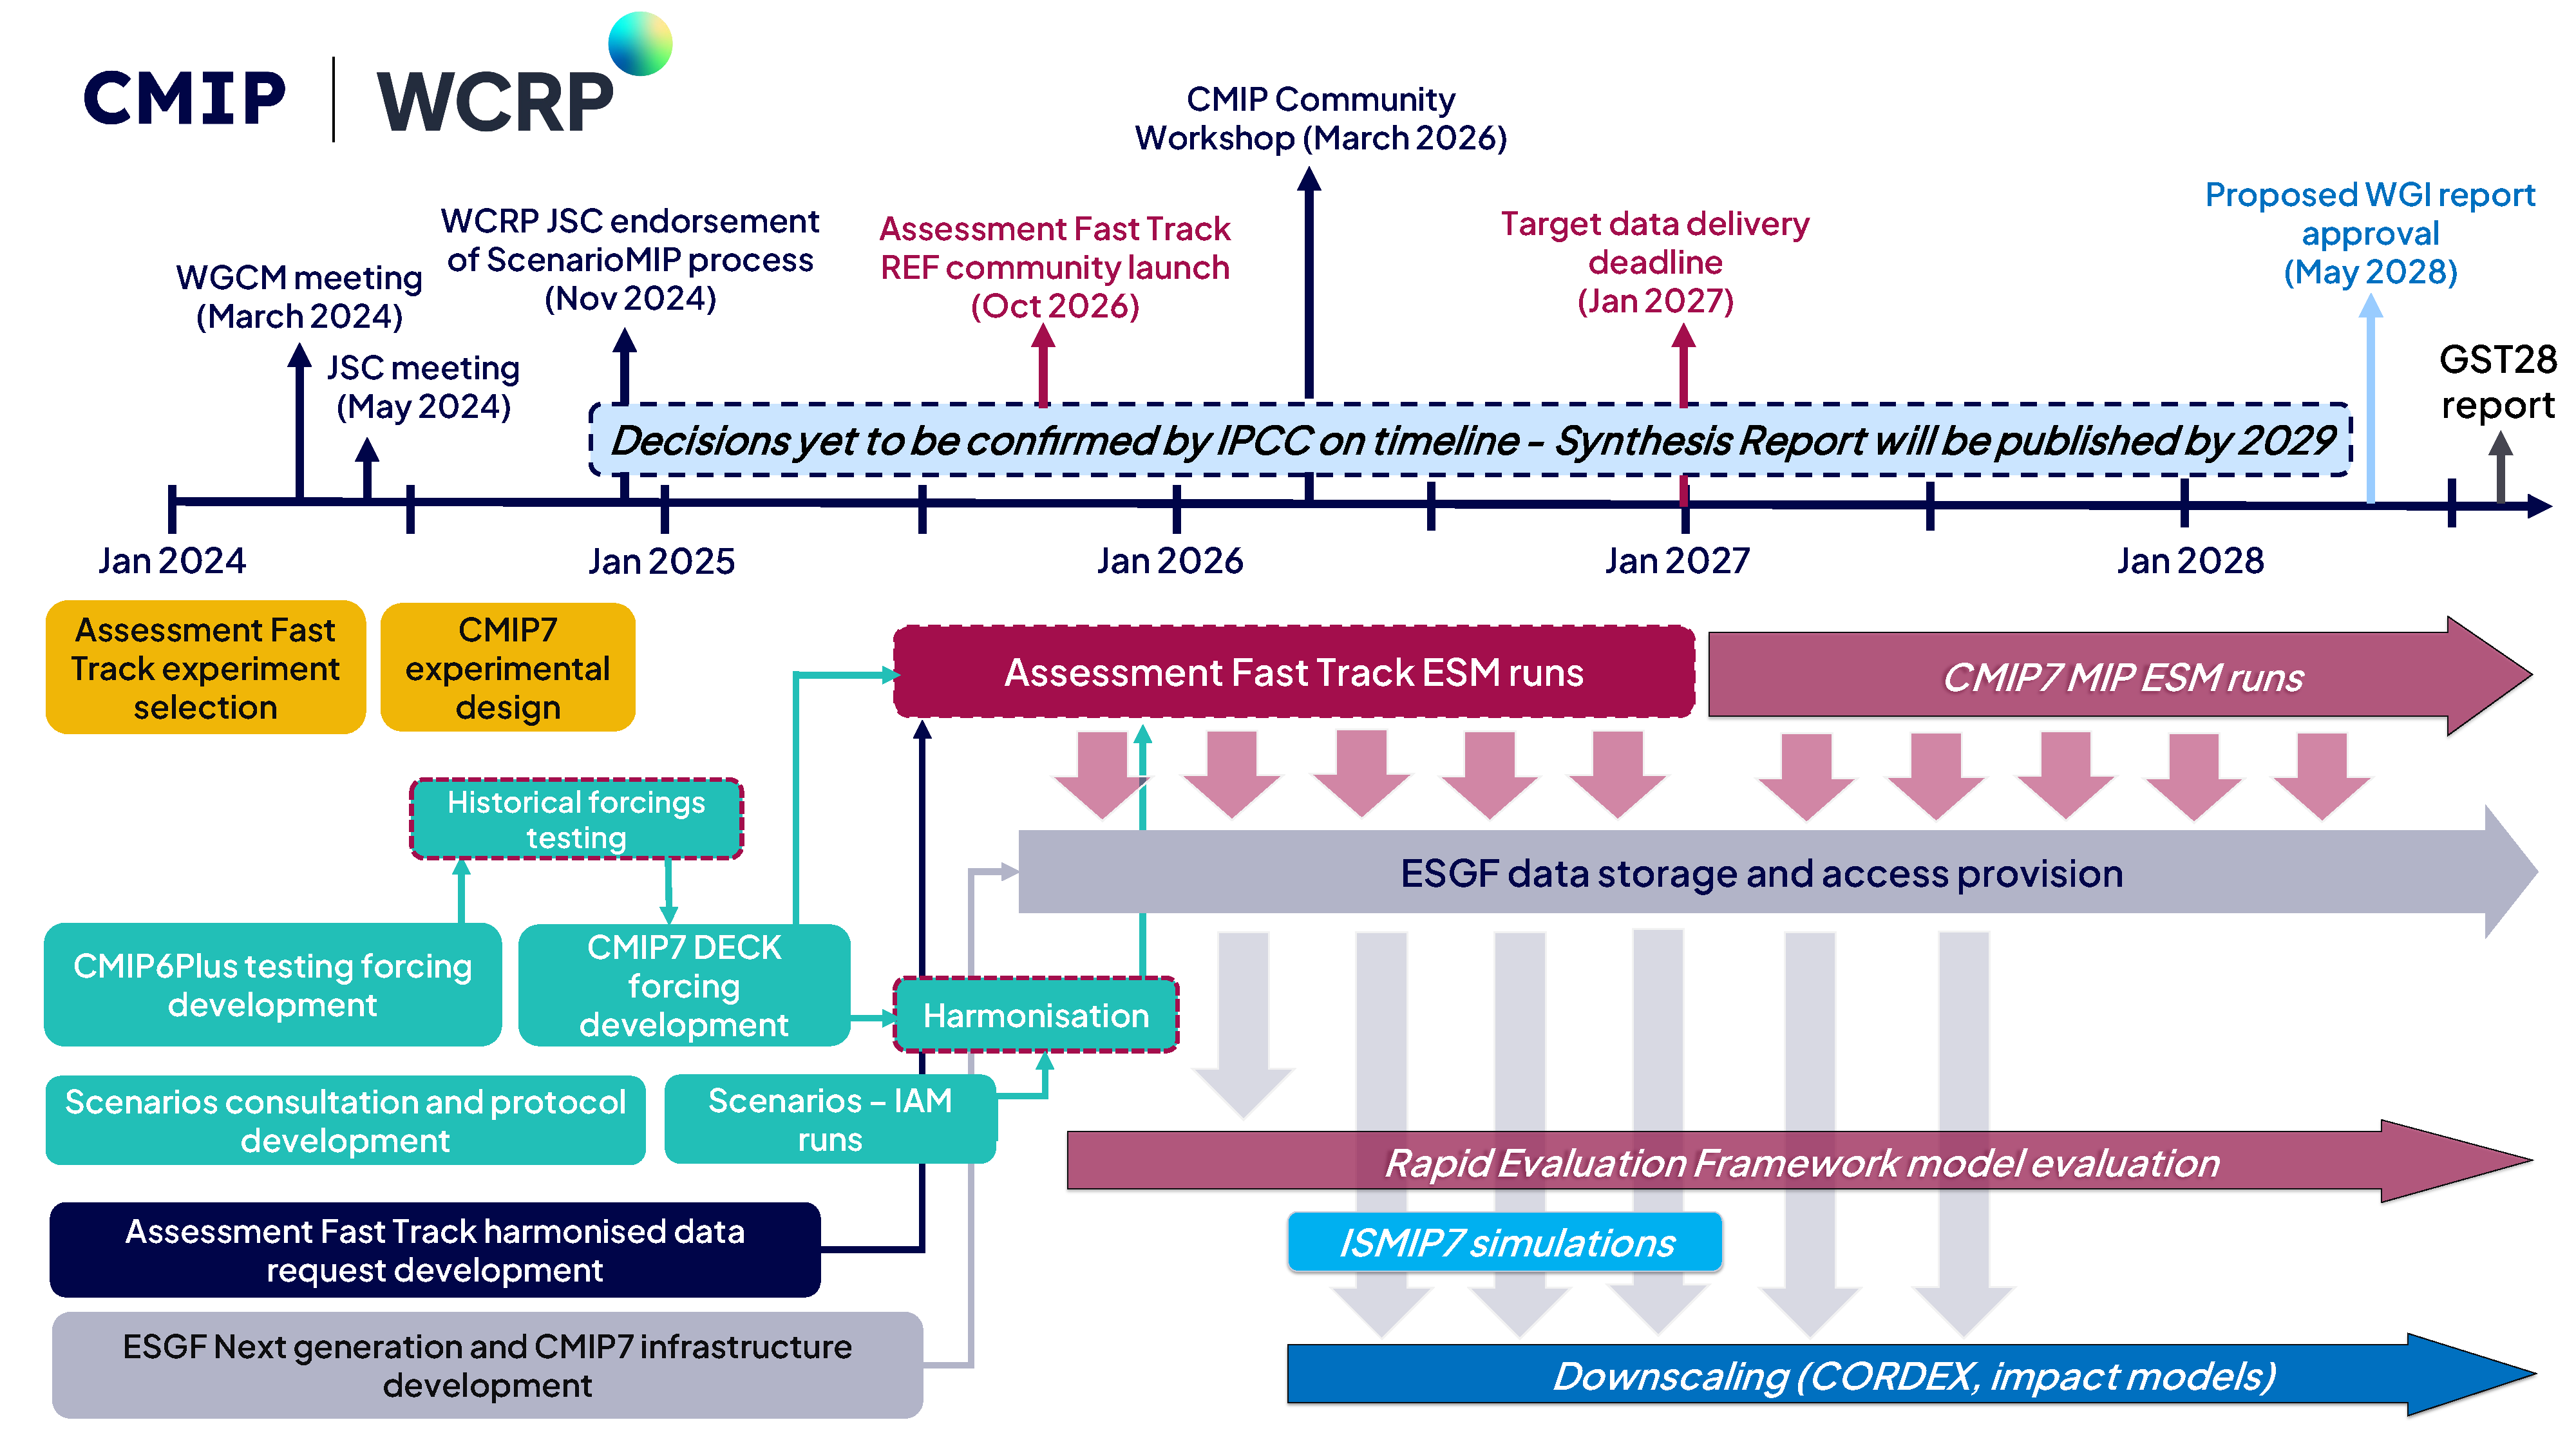
\includegraphics[width=\textwidth,angle=0]{250515_Fig1.pdf}\\
	 \caption{Timeline of the CMIP7 planning and progress - Climate forcings are essential inputs that enable modeling groups to initiate pre-industrial control and historical simulations (latest figure version is available at https://doi.org/10.5281/zenodo.15230117). \cred{Note typo - Assessment Fast Track REF community launch Oct 2026/should be Oct 2025)}}
	 \label{fig:f1}
\end{figure}


\section*{Goal 1: Latest climate-forcing dataset evaluation in preparation for CMIP7}
The first two days discussed dataset progress. Many datasets evolved from CMIP6 precedents, and new data have largely recognized and resolved identified issues during the CMIP6 and CMIP6Plus reviews. These data are now available for CMIP7 simulations to commence (Table 1).

Session one focused on latest-generation data updates. Summaries were provided for the solar, land use change, and stratospheric volcanic aerosol forcing datasets, all of which have undergone significant revisions since CMIP6. The Fresh Eyes on CMIP, a group of early career researchers, assessed early CMIP6Plus prototype datasets, providing comparisons between the preceding CMIP6- and developing data. They highlighted several issues addressed in the final data releases (Table 1). Additional discussion on forcings of the paleoclimate warm last interglacial and similar deep time periods occurred. Plans were defined to harmonize these PMIP forcings ($>$100k years earlier than present) with those covering the Holocene to the present day. All new datasets extend to 2022/2023/2024, an additional decade on the CMIP6-era data (2014 CMIP6’s last year), and offer similar spatial resolutions as preceding datasets.

In session two, discussions shifted from the recently observed past to future ScenarioMIP scenario development plans \citep{van_vuuren_scenario_2025}. First, there were plans describing the alignment of historical and scenario data, focusing on anthropogenic emissions, associated concentrations, and land-use changes, along with scenario extensions past 2100. Next, the recent experience of the European RESCUE project (https://rescue-climate.eu) was described. RESCUE is one of the first projects to define scenarios, including numerous carbon dioxide removal (CDR) methods for ESMs. The second-to-last talk introduced new ESM diagnostics, which are required to ensure accurate carbon accounting is achieved. We concluded the session with a CMIP7 ScenarioMIP plan summary, highlighting the seven illustrative scenarios, with all but one showing flat or decreasing anthropogenic GHG future emissions \citep{van_vuuren_scenario_2025}.

\subsubsection*{From Earth’s observed history to the future [potential inset box format]}
Before reviewing the CMIP7 forcing status, it's essential to highlight ongoing efforts to develop future scenario forcings, which run in parallel with the refinement of historical datasets. ScenarioMIP \citep{van_vuuren_scenario_2025} defines these scenarios, initially quantified by integrated assessment models (IAMs). IAM outputs are then passed to forcing teams, who harmonize the data—ensuring smooth transitions from historical to future periods—and generate the forcings used by ESMs. These standardized datasets enable experiments spanning Earth’s past (1850–2021) to potential futures (2022–2125) and are expected to be released in July 2025 (Figure 1).

\section*{Goal 1: Latest climate-forcing dataset evaluation in preparation for CMIP7 (continued)}
The second day shifted gears. Session three focused on CMIP7 ``Diagnostic, Evaluation and Characterization of Klima'' (DECK; i.e., core experiments) protocol development. We heard from NOAA-GFDL, NCAR, and CSIRO modelers, who reported test simulation feedback with prototype CMIP6Plus datasets, along with CMIP6 data differences, and identified issues that were subsequently resolved. The consensus was that the new data reproduced the same results as the previous CMIP6 data; however, the latest data provided more information, including enhanced variability quantification and more comprehensive event coverage, particularly over the well-sampled satellite period.

Targeted talks addressed updates to volcanic, solar, and biomass-burning datasets in the context of forcing implementation for the piControl and future scenario experiments. For volcanic forcing, the uneven timing of eruptions complicates defining a representative pre-industrial climatology and incorporating volcanoes into future scenarios. While the satellite era is well constrained, the new dataset integrates additional ice core and geological records, expanding coverage and increasing uncertainty in event magnitude and location. Solar forcing, active in models for decades, has seen total solar irradiance (TSI) estimates vary by $\sim$0.5\% since AMIP began in 1989 \citep{durack_coupled_2025}. The latest dataset has been enhanced to support high-top atmospheric models that simulate the mesosphere and lower thermosphere, which are particularly relevant for ozone modeling. An update to biomass-burning emissions was also presented, noting a step change in Northern Hemisphere variability in 1997 in the CMIP6-era dataset that induced anomalous warming across three ESMs \cite[e.g.,][]{fasullo_overview_2024,holland_new_2024}. These talks underscored the need for continued dataset refinement and better uncertainty quantification in future experiments.

Next, a virtual forcings drop-in session was held, providing engagement and discussion between the forcing providers and the CMIP modeling teams. Many issues were covered, with the most widely discussed being the provision of pre-industrial control (piControl) forcings. These are the key first step for modeling centers to spin up, finalize development, and freeze their CMIP7 model configurations.

In session four, we covered past forcing issues, uncertainties, a case study on implementing forcing data in ESMs, and missing datasets in the CMIP7 DECK protocol \citep{dunne_evolving_2024}. We reviewed how the progression of forcing data and model development has been closely tied, with growing model complexity driving increased demands for detailed and voluminous forcing data. The CMIP6 example of late changes to sulfate emissions in China highlighted the need for a responsive and adaptable approach, informing CMIP7’s more consultative delivery strategy. We also saw research comparing forcing datasets across two CMIP6 modeling groups, showing that changes in forcings can impact climate outcomes as much as model version differences \citep{fyfe_significant_2021,holland_new_2024}. The session underscored the central role of forcings in ESM development and the many open questions in this field.

From the modeling team perspective, IPSL described how CMIP6-era forcings were implemented to construct their simulation suite. Significant customization was required to reformat the data for model use, and updates to earlier forcings necessitated retuning to align with observations \citep{lurton_implementation_2020}. The talk emphasized the ongoing need for more precise documentation of how ESM teams prepare and apply forcings, as even small implementation choices can lead to notably different climate outcomes. It also highlighted further opportunities for data evolution, with the potential to identify common reformatting procedures and implement them in the data development steps. 

The session then shifted to forcing datasets currently missing but needed to support evolving or absent process representations in models. First was the simple plumes parameterization—used since CMIP6 to account for aerosol radiative effects in models lacking explicit aerosol transformation schemes \citep[e.g.,][]{stevens_macv2-sp_2017,fiedler_anthropogenic_2019}. Next, the increasing freshwater input from glaciers and ice sheets was discussed. Often missing in models without interactive ice sheets, this forcing significantly influences Southern Ocean responses and is a known gap in current protocols \citep[e.g.,][]{roach_winds_2023,schmidt_anomalous_2023}. Groundwater irrigation was also highlighted—irrigated land has nearly tripled since 1950, affecting the near-surface climate through changes in soil moisture. Biomass burning emissions followed, with concerns about outdated pre-industrial estimates and the omission of climate-driven fire regime changes in future scenarios \citep[e.g.,][]{chen_multi-decadal_2023,hamilton_global_2024}. These omissions could introduce radiative forcing uncertainties of ~1–2 W/m² from the pre-industrial era to today \citep{hamilton_reassessment_2018,wan_importance_2021}.

The final session addressed several unmet modeling needs. These included human population and development density for estimating interactive fire ignitions; the omission of hydrogen’s global warming potential from current scenarios \citep[e.g.,][]{sand_multi-model_2023}; and the underestimation of aeolian dust, highlighted by comparison with recent reconstructions \citep[e.g.,][]{kok_mineral_2023}.

By the conclusion of the first two days, it was clear that substantial work is still needed to improve confidence in climate forcings. To create a consistent historical timeline, a key challenge is bridging the sparse pre-satellite record with the better-sampled modern era. New CMIP7 datasets reveal significant shifts across data stream transitions, especially for volcanic aerosols and biomass burning, emphasizing historical uncertainties. Another issue is determining the vertical injection height for anthropogenic emissions, which remains difficult even in the satellite era. Emerging research suggests that uncertainty in emission injection height has a large impact on model results, potentially affecting aerosol climate impact estimates \citep[e.g.,][]{ahsan_emissions_2023}.

In parallel, as models grow more complex, their forcing requirements increase. Many CMIP7 models in development plan to run in emissions mode—using point-source emissions instead of well-mixed concentrations—further raising the demand for detailed forcing data. Meeting these evolving needs will require continued efforts to better quantify uncertainties and improve the consistency of historical estimates.

\section*{Goal 2: From next-generation evolution to sustained revolution}
For the last two days, the meeting shifted to its second goal: the future of forcings. The aim was to recognize and document the limited support for current activities, to identify new key opportunities for future forcing development in a sustained mode and funding, and to revisit the reach and use of these datasets across an expanding user base.

Session six began with a review of current data contributors, their observational data streams, and the support structures in place for them. Over 20 funding sources across multiple countries were identified, including national agencies, consortia, commissions, and individual institutions supported by grants and philanthropic funding. Opportunities for improvement included better sharing of tools and knowledge, as well as leveraging existing CMIP infrastructure.

The session then moved into plenaries and active discussion. The first plenary outlined downstream users—both within the World Climate Research Program (WCRP) and more broadly across the World Meteorological Organization (WMO)—and their varied needs for weather, seasonal prediction, and climate information. Brief presentations followed, showcasing the diversity of user requirements and parallel efforts to generate forcing data for recent and regional contexts. CMIP’s long historical coverage (to 1850) was described as the ``gold standard,'' while many alternative datasets are in use for the well-observed modern satellite era. Talks also emphasized the growing demand for higher-resolution forcings across applications, including CORDEX downscaling, ECMWF seasonal forecasts, decadal predictions, Copernicus, and DestinE, with the new insight that many of these seasonal-decadal forecast and reanalysis activities are already leveraging existing CMIP forcing data. Related global efforts such as the Global Carbon Project \citep{friedlingstein_global_2024} and Indicators of Global Climate Change \citep{forster_indicators_2024} were also discussed.

A key idea emerged from the discussions: while continued scientific exploration of forcings is vital, many users also need routinely produced, stable datasets. This led to the concept of updates and extensions. Updates involve revising entire datasets, including past data, to reflect new knowledge, supporting scientific progress. Extensions add only recent data without altering earlier values, which is critical for operational users, such as weather prediction centers. Balancing these needs will require new approaches, as few current workflows or funding opportunities effectively support both of them.

Plenary two focused on the challenges of establishing more routine forcing production, beginning with an overview of the CMIP Forcings Task Team and its funding model. An open panel followed, featuring representatives from key international agencies—including ESA, ECMWF, NOAA, the U.S. DoE, and the European Commission. Panelists strongly supported the continued development of climate forcing datasets to meet growing demands. However, they also noted that legislative mandates and agency coordination requirements often constrain how funding can be allocated, limiting flexibility to support all user needs.

Plenaries three and four transitioned into breakout sessions, where participants explored user needs, current working models, and funding status to help define a path toward sustained forcing data delivery. The final plenary session summarized key takeaways and outlined next steps, emphasizing the importance of publishing these insights to initiate broader coordination and support long-term, sustained Earth system forcing efforts.

\section*{Status and community next steps}
Preparations for the Coupled Model Intercomparison Project Phase 7 (CMIP7) are progressing, with a major milestone now achieved—the delivery of updated ``forcing'' datasets. These datasets are critical Earth System Model (ESM) inputs, guiding climate simulations in response to historical natural and anthropogenic changes. The ``Pathway to Regular and Sustained Delivery of Climate Forcing Datasets'' workshop brought together a broad community to advance CMIP7’s objectives. It also laid the groundwork for long-term planning, aiming to establish a sustainable framework for the ongoing provision of forcing datasets to support CMIP7, follow-on activities, and a wide range of weather and climate science applications.

The meeting produced two key outcomes. First, it refined CMIP7 plans, reviewed prototype data, and outlined the delivery of forcing datasets while identifying areas for improvement and future development. More importantly, it recognized that these datasets have grown beyond their original role of standardizing model inputs, becoming foundational across Earth system science, with impact and use significantly broader than their CMIP project origins. As their use broadens across disciplines and timescales, expectations of data producers are shifting—underscoring the need to evolve collaboration models and funding structures. A central theme emerged: forcing datasets must keep pace with scientific demands to ensure robust, consistent climate and weather information. Such evolution will unlock new opportunities and strengthen the foundation for advancing Earth system science.

The workshop identified key actions to maintain CMIP7 momentum, including clarifying funding support for existing forcing providers, mapping dataset interdependencies, and assessing funding agency engagement in consideration of global political dynamics. These tasks will be shared by the CMIP Forcings Task Team and the workshop committee over the coming year, supporting both CMIP7 delivery and long-term Earth System Science planning.


\clearpage
%%%%%%%%%%%%%%%%%%%%%%%%%%%%%%%%%%%%%%%%%%%%%%%%%%%%%%%%%%%%%%%%%%%%%
% ACKNOWLEDGMENTS
%%%%%%%%%%%%%%%%%%%%%%%%%%%%%%%%%%%%%%%%%%%%%%%%%%%%%%%%%%%%%%%%%%%%%
\acknowledgments
The authors would like to thank all members of the CMIP Forcing Task Team for their tireless efforts making CMIP7 forcing datasets a reality, the ``team'' includes: Thomas Aubry, Louise Chini, John Fasullo, Stephanie Fiedler, Bernd Funke, Heather Graven, Michaela Hegglin, Jarmo Kikstra, Thibaut Lurton, Claire MacIntosh, David Plummer, Steven Smith, Margreet van Marle, Tilo Ziehn, Keywan Riahi, Guido van der Werf, Rachel Hoesly, Mahesh Kovilakam, Ken Mankoff, Malte Meinshausen, Anja Schmidt, Doug Smith and Tim Stockdale. The CMIP Forcing Task Team homepage can be viewed at \url{https://wcrp-cmip.org/cmip7-task-teams/forcings}. The authors would also like to thank the European Centre for Medium-Range Weather Forecasts (ECMWF), Copernicus Climate Change Service (C3S), and the European Space Agency (ESA) for jointly hosting and sponsoring the workshop. We recognize the CMIP International Project Office (CMIP-IPO) staff, hosted by ESA, and the staff provided on contract by HE Space Operations Ltd., for their exceptional workshop organization and execution. We recognize numerous international agencies supporting data development. The work of P.J.D. from Lawrence Livermore National Laboratory (LLNL) is supported by the Regional and Global Model Analysis (RGMA) program area under the Earth and Environmental System Modeling (EESM) program within the Earth and Environmental Systems Sciences Division (EESSD) of the United States Department of Energy’s (DoE) Office of Science. This work was performed under the auspices of the US DoE by LLNL under contract DE-AC52-07NA27344. LLNL IM Release: LLNL-JRNL-2002809. ZN acknowledges financial support by the CMIP International Project Office (CMIP IPO), which is hosted by the European Space Agency (ESA) as part of the GHG Forcing For CMIP project of the Climate Change Initiative (CCI) (ESA Contract No. 4000146681/24/I-LR-cl) and the European Union's Horizon 2020 research and innovation programmes (grant agreement no. 101003536) (ESM2025). HH is supported by the Met Office Hadley Centre Climate Programme funded by the Department for Science, Innovation and Technology (DSIT), UK.


%%%%%%%%%%%%%%%%%%%%%%%%%%%%%%%%%%%%%%%%%%%%%%%%%%%%%%%%%%%%%%%%%%%%%
% DATA AVAILABILITY STATEMENT
%%%%%%%%%%%%%%%%%%%%%%%%%%%%%%%%%%%%%%%%%%%%%%%%%%%%%%%%%%%%%%%%%%%%%
\datastatement
No data was generated in the production of this Meeting Report. Presented materials referred to in this document can be accessed from the workshop website at \url{https://wcrp-cmip.org/event/forcings-workshop/}.


%%%%%%%%%%%%%%%%%%%%%%%%%%%%%%%%%%%%%%%%%%%%%%%%%%%%%%%%%%%%%%%%%%%%%
% REFERENCES
%%%%%%%%%%%%%%%%%%%%%%%%%%%%%%%%%%%%%%%%%%%%%%%%%%%%%%%%%%%%%%%%%%%%%
% Make your BibTeX bibliography by using these commands:
\bibliographystyle{ametsocV6}
\bibliography{250515c}

\end{document}